\section{The Background Channels}
% The dominant SM backgrounds can be divided into two categories: (i) from leptonic $\tau$ decays and (ii) from fake leptons. In the first category, the dominant process is the pair production of $W Z$ with $W$ decaying leptonically and $Z \rightarrow \tau \tau$. The trilepton final states with no-OSSF pairs can arise from the subsequent leptonic decay of $\tau$ 's. We estimate this background process via Monte Carlo simulations.
% \\
% The dominant processes of the second category are $\gamma^{*} / Z+$ jets and $t \bar{t}$, where two leptons come from $\gamma^{*} / Z \rightarrow \tau \tau$ or the prompt decay of $t$ and $\bar{t}$, and a third lepton is faked from jets containing heavy-flavor mesons.
We define background as anything that is not of interest. As will be further explained in  later sections,
we will explicitly demand a 3-lepton final-state in all collisions considered in the analysis. This will 
remove a lot of background, but not all. Due to the imperfect nature of the reconstruction of events,
a demand for 3-lepton final-state will not be without errors. This leaves room for more variation in 
the background than one might expect. In this section I will cover the channels\footnote{By channels,
we refer to the physical diversity which could lead to a specific final-state. Often this refers to 
the different particles which mediates the process from initial- to final-state.} which will 
be of importance during the analysis. I will also discuss which background channels are the hardest 
to reduce in a potential signal region, also called the irreducible background. These are 
channels whom exhibit similar trends/distribution in the features. Note that the sections bellow
are listed by contribution to the data (from most to least).  

\subsection{Z-jets}
The Z-jets channel is the largest contribution in all the data. The channel consists of all events
resulting in a Z-boson alongside jets. In the cases the Z-boson decays to two leptons, the additional 
jet acts as a fake lepton and the channel classifies as a 3-lepton final state. In figure \ref{fig:z_pjets} 
I have written the Feynman diagram of an example of such a channel. The figure shows two quarks decaying 
into a Z-boson and gluon, mediated by a third quark. The Z boson decays into two leptons (normally 
$e^-e^+$ or $\mu^- \mu^+$) and the gluon decays to a pair of bottom quarks which act as a fake lepton. 
\begin{figure}
    \centering
    \makebox[0.75\linewidth][c]{%
    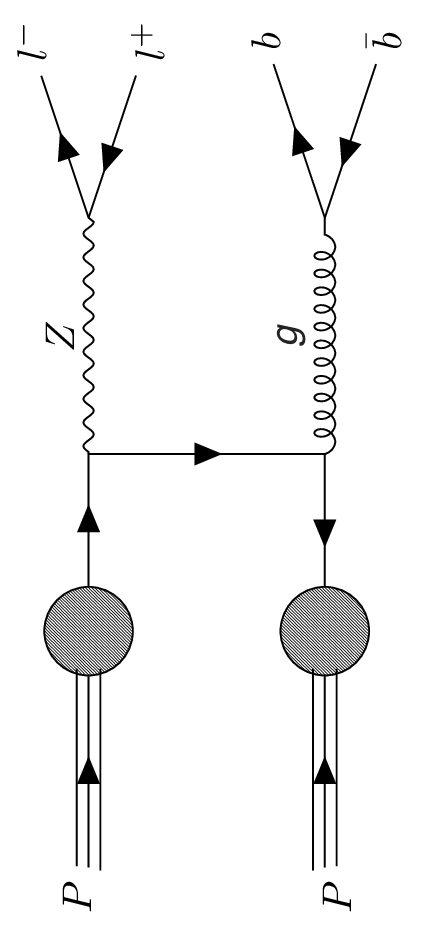
\includegraphics[width=0.225\textwidth, angle = -90]{Figures/FDiagrams/Z_pjets.png}
    }
    \caption{The Feynman diagram of the  Z-jets channel.}
    \label{fig:z_pjets}
\end{figure}

\subsection{Diboson (lll)}
Dibson channels are defined as channels resulting in two bosons. In the case of (lll), the dibosons
decay into a total of three leptons. In figure \ref{fig:wz} I have drawn the Feynman diagram of an 
example of such a channel. The figure shows two quarks decaying into a W- and Z-boson through a 
third quark. The W-boson decays into a pair of charged and neutral lepton and the Z-boson decays 
into a pair of leptons. 
\begin{figure}
    \centering
    \makebox[0.75\linewidth][c]{%
    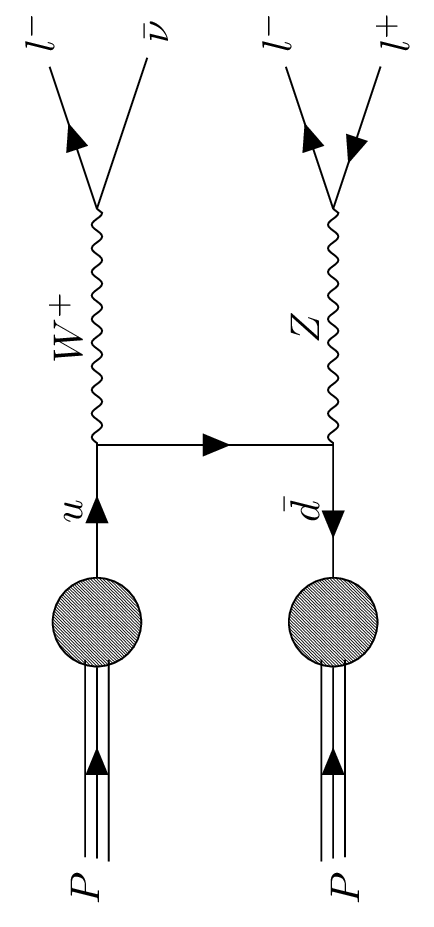
\includegraphics[width=0.225\textwidth, angle = -90]{Figures/FDiagrams/wz.png}
    }
    \caption{The Feynman diagram of the diboson WZ-channel.}
    \label{fig:wz}
\end{figure}
\subsection{$t\bar{t}$}
The $t\bar{t}$ channel is defined as a channel resulting in a pair of top quarks. In figure
\ref{fig:ttbar} I have drawn a Feynman diagram of an example of such a channel. The figure 
shows two gluons decaying into a pair of top quarks, mediated by a third. The two top quarks 
decay into a jet and two leptons with missing energy (neutrinos). 
\begin{figure}
    \centering
    \makebox[0.75\linewidth][c]{%
    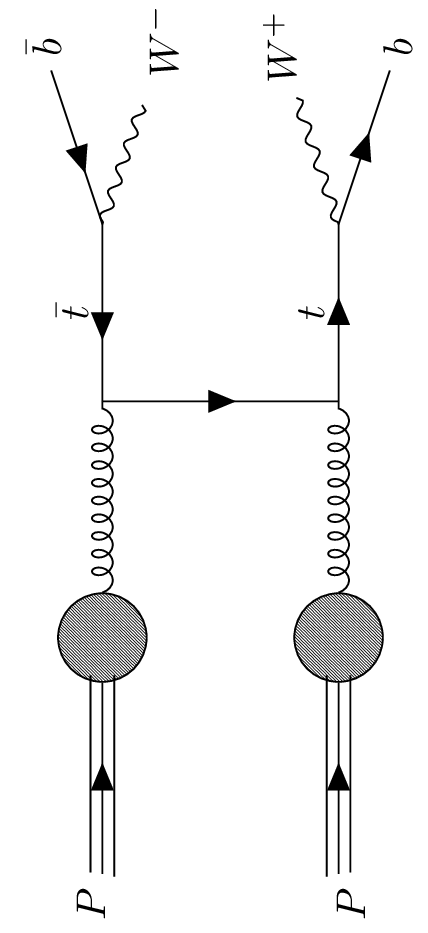
\includegraphics[width=0.225\textwidth, angle = -90]{Figures/FDiagrams/ttbar.png}
    }
    \caption{The Feynman diagram of the $t\bar{t}$-channel.}
    \label{fig:ttbar}
\end{figure}

\subsection{Diboson (llll)}
In the case of diboson (llll), the channel refers to events resulting in two bosons which decay 
into four leptons. In figure \ref{fig:zz} I have drawn a Feynman diagram of an example of 
such a diagram. The figure shows two quarks decaying into two Z-bosons through a third quark.
The two Z-bosons decay into two pairs of leptons. 
\begin{figure}
    \centering
    \makebox[0.75\linewidth][c]{%
    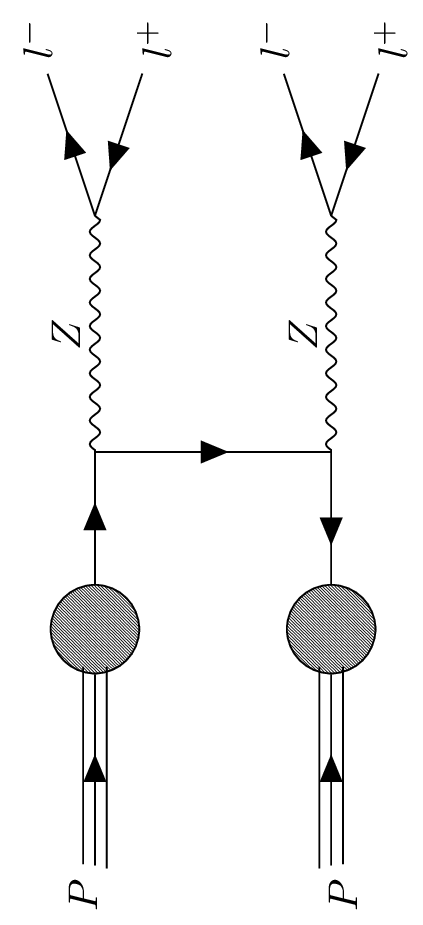
\includegraphics[width=0.225\textwidth, angle = -90]{Figures/FDiagrams/zz.png}
    }
    \caption{The Feynman diagram of the ZZ-channel.}
    \label{fig:zz}
\end{figure}



\subsection{Top Others}
\subsection{Single Others}
\subsection{Diboson (ll)}
\subsection{Others}

\begin{figure}
    \centering
    \makebox[0.75\linewidth][c]{%
    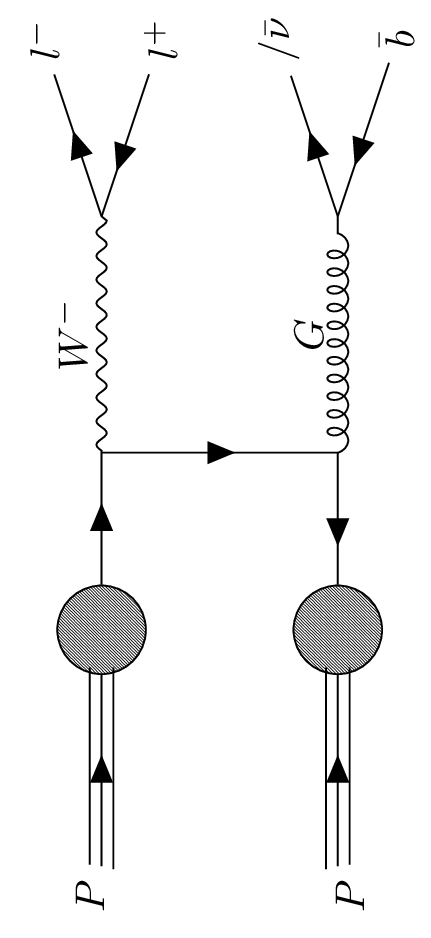
\includegraphics[width=0.225\textwidth, angle = -90]{Figures/FDiagrams/w_pjets.png}
    }
    \caption{The Feynman diagram of the diboson W-jets channel.}
    \label{fig:w_pjets}
\end{figure}
\begin{figure}
    \centering
    \makebox[0.75\linewidth][c]{%
    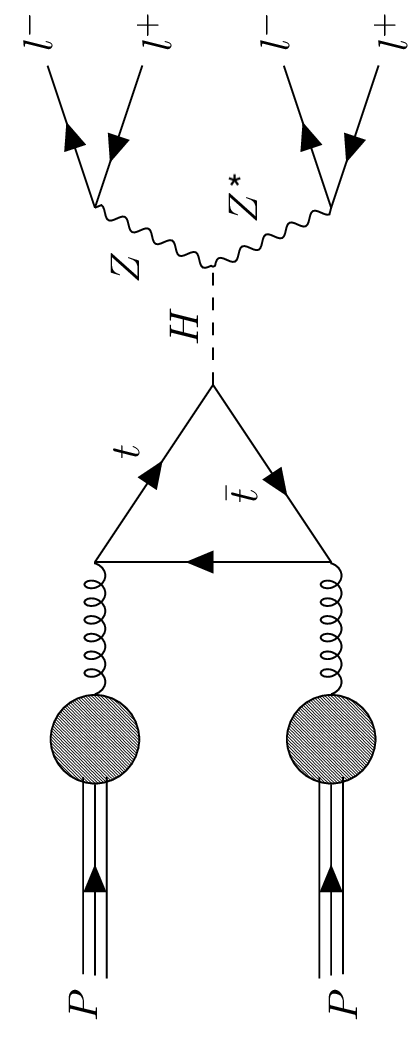
\includegraphics[width=0.225\textwidth, angle = -90]{Figures/FDiagrams/h.png}
    }
    \caption{The Feynman diagram of the Higgs-channel.}
    \label{fig:h}
\end{figure}
\begin{figure}
    \centering
    \makebox[0.75\linewidth][c]{%
    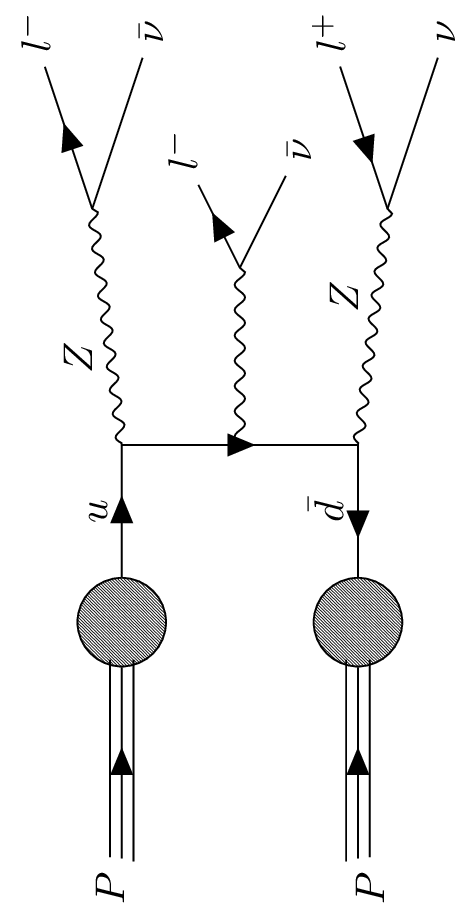
\includegraphics[width=0.225\textwidth, angle = -90]{Figures/FDiagrams/zzz.png}
    }
    \caption{The Feynman diagram of the Triboson-channel.}
    \label{fig:zzz}
\end{figure}
